\subsubsection{Recursion}

\YIComment{Redo this}

\autoref{figure:fibonacci-mips} shows the performance of the \texttt{fibonacci(n)} test suite. It has a very similar performance characteristic to the \texttt{primal(n)} test suite with some notable differences.

The overall performance for both SUTs is significantly lower. This is due to the memory instructions required for pushing and popping the stack, which have much lower emulation performance compared to arithmetic instructions.

The JIT emulator takes significantly longer to reach peak performance whereas the interpreter does not. This is because the interpreters fixed costs, such as initialization, do not change with the program being executed. The JIT emulator on the other hand has additional costs for every block that needs compiling, and the \texttt{fibonacci(n)} program contains more source blocks. This means there is a larger initial cost which takes longer to amortize.

\begin{figure}[H]
    \centering
    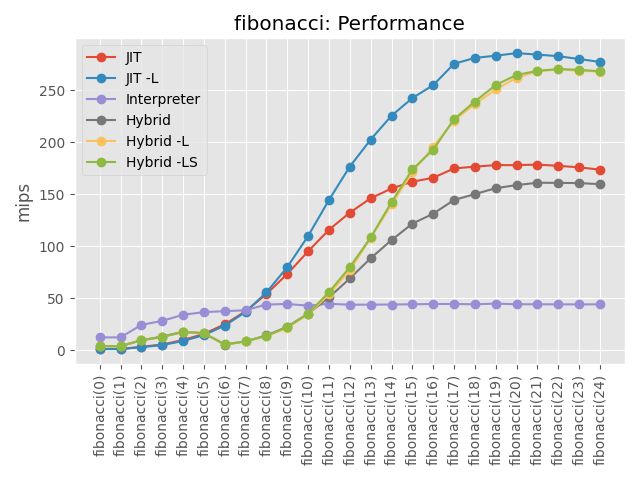
\includegraphics[scale=0.75]{output/graphs/tests/all/fibonacci/mips.png}
    \caption{Performance in mips of the fibonacci test suite.}
    \label{figure:fibonacci-mips}
\end{figure}